\section{DrQA}
\subsection{Tổng quan}
Mục tiêu của DrQA là trả lời các câu hỏi thuộc dạng open-domain. DrQA sử dụng nguồn dữ liệu từ
Wikipedia làm cơ sở tri thức (knowledge base).

\begin{figure}[h!]
    \centering
    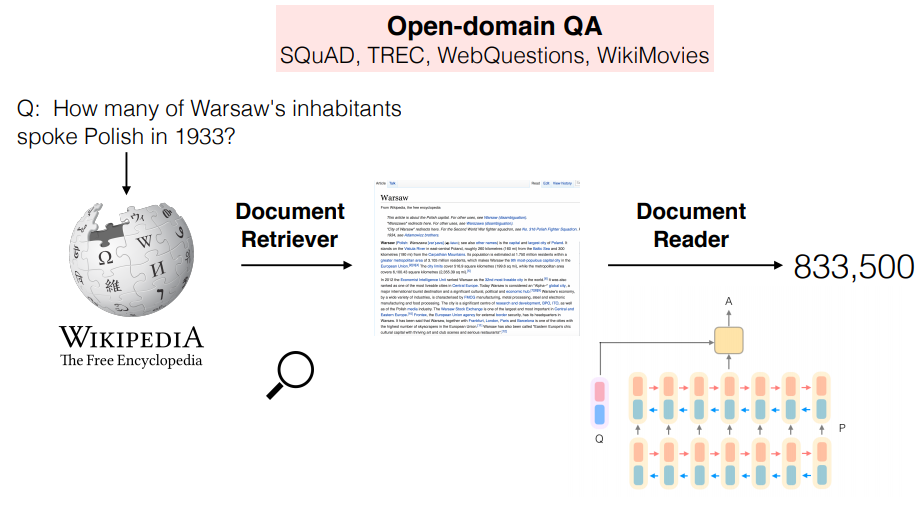
\includegraphics[scale=0.5]{drqa-overview.jpg}
    \caption{Tổng quan về hệ thống DrQA}
    \label{fig:my_label}
\end{figure}

Phương pháp bao gồm 2 phần chính là bộ lấy tài liệu (Document Retriver) và bộ đọc tài liệu (Document Reader). Trong đó
\begin{enumerate}
    \item \textbf{Document Retriever} thu hẹp phạm vi tìm kiếm, từ tập các tài liệu (document) ban đầu, lấy ra một tập nhỏ các tài liệu có liên quan nhất. Cụ thể với DrQA, tập tài liệu là tập các bài viết trên Wikipedia, Document Retriever sẽ lấy ra  k = 5 tài liệu liên quan nhất đến câu hỏi.
    \item \textbf{Document Reader} nhận đầu vào là tập các bài viết liên quan được lấy ra từ bước Document Retriever, sau đó tìm ra đoạn văn có khả năng cao nhất là đáp án. 
\end{enumerate}

\subsection{Document Retriever}
DrQA sử dụng cách đánh giá bằng TF-IDF, một phương pháp hiệu quả được sử dụng trong các công cụ tìm kiếm (search engine) mà không cần qua quá trình học. TF-IDF là viết tắt của term frequency - inverted document frequency. Giá trị này xuất phát từ một nhận xét rằng: một từ sẽ càng có ý nghĩa với việc tìm kiếm nếu nó xuất hiện nhiều lần trong một tài liệu, và nó chỉ xuất hiện trong một số ít các tài liệu.\\
Để tính toán giá trị này, trước tiên, truy vấn và  các tài liệu được chuyển về dưới dạng vector bag-of-word. Mỗi từ \textit{t} ứng với tài liệu \textit{d} và tập tài liệu \textit{D} sẽ được tính giá trị tf-idf như sau:
\begin{gather*}
    tfidf(t, d, D) = tf(t, d) \times idf(t, D) \\ 
    tf(t, d) = log(1 + freq(t, d))\\ 
    idf(t, D) = \log \frac{|D|}{|d \thinspace \in \thinspace D \thinspace : \thinspace t \thinspace \in \thinspace d|} 
\end{gather*}

Với $freq(t, d)$ là số lần từ $t$ xuất hiện trong tài liệu $d$. $t$ ở đây có thể là unigram hoặc bigram term.
DrQA sử dụng một tokenizer để thực hiện phân đoạn câu cũng như xác định từ loại cho các từ trong câu. Đối với một tài liệu $d$, giá trị của tài liệu đối với truy vấn $q$ được tính như sau:
\begin{gather*}
    score(q, d) = \sum_{t \thinspace \in \thinspace q}^{} tfidf(t, d).    
\end{gather*}
DrQA mặc định lấy ra $k = 5$ tài liệu có điểm số cao nhất với câu hỏi.


\subsection{Document Reader}
Document reader sẽ nhận đầu vào là một câu hỏi q được biểu diễn dưới dạng $ \{q_1, q_2, ..., q_l\} $ với l là số tokens ở trong câu hỏi và một tập các tài liệu. Trong đó, mỗi tài liệu được chia thành các đoạn văn, mỗi đoạn văn p được biểu diễn bởi  $\{p_1, p_2, ..., p_m\} $ với m là số tokens của đoạn văn. Mô hình document reader sẽ có 3 phần chính: paragraph encoding, question encoding và prediction.

\subsubsection{Paragraph Encoding}
Ta biểu diễn các token $p_i$ dưới dạng một vector đặc trưng $\tilde{p_i}$. Vector đặc trưng $\tilde{p_i}$  bao gồm những thành phần sau:

\begin{itemize}
    \item Word embedding: $f_{emb}(p_i) = E(p_i)$. Glove word embedding được sử dụng để thực hiện việc embedding. Đa số các từ pre-trained word embedding đều được cố định và chỉ thực hiện fine-tune 1000 từ thường xuyên xuất hiện nhất. 
    \item Exact match: $f_{exact\_match}(p_i) = \Pi(p_i \in q)$. Sử dụng 3 binary features để biểu diễn $p_i$ có khớp với một từ ở trong câu hỏi $q$, có thể ở dạng ban đầu (giống như trong câu hỏi), không phân biệt chữ hoa, thường (case-insensitive), hoặc ở dạng nguyên bản (lemma form, ví dụ như các từ break, breaks, broke và broken có chung dạng nguyên bản là break).
    \item Đặc trưng của token: $f_{token}(p_i) = (POS(p_i), NER(p_i), TF(p_i))$. Các đặc trưng về từ loại (POS - part of speech), loại thực thể của các đối tượng có tên (NER - named entity recognition), và tần suất xuất hiện của từ (TF - term frequency). 
    \item Aligned question embedding:
    $f_{align}(p_i) = \sum_j a_i_j E(q_j)$, trong đó trọng số attention $a_i_j$ thể hiện sự gióng hàng (alignment) giữa $p_i$ và mỗi từ $q_j$ trong câu hỏi. Cụ thể, $a_i_j$ được tính bằng tích chấm giữa các ánh xạ phi tuyến (nonlinear mappings) của các word embedding:
    \begin{gather*}
        a_i_j = \frac{exp(\alpha(E(p_i)) \cdot \alpha(E(q_j)))}{\sum_{j'} exp(\alpha(E(p_i)) \cdot \alpha(E(q_{j'})))}
    \end{gather*}
    trong đó $\alpha()$ là một lớp fully-connected với hàm activation phi tuyến ReLU. So với đặc trưng exact match, đặc trưng này bổ sung thêm các gióng hàng tương đối (soft alignment) giữa các từ tương tự nhưng không giống nhau (ví dụ: car và vehicle). 
\end{itemize}

Tập vector đặc trưng $\tilde{p}_{1}, \tilde{p}_{2}, \dots, \tilde{p}_{m}$ sau đó sẽ được đưa qua LSTM để thu được:
\begin{gather*}
   \{\textbf{p}_{1}, \textbf{p}_{2}, \dots, \textbf{p}_{m}\} = RNN(\{\tilde{p}_{1},\tilde{p}_{2}, \dots, \tilde{p}_{m}\})
\end{gather*}
với $\textbf{p}_{i}$ được kì vọng sẽ mã hóa các thông tin về ngữ cảnh.

\subsubsection{Question Encoding}
Câu hỏi $q$ được encode thành tổng có trọng số của các từ trong câu hỏi. Cụ thể, vector $\textbf{q}$ được biểu diễn dưới dạng $\textbf{q} = \sum b_j \times q_j$, trong đó $b_j$ thể hiện độ quan trong của mỗi từ trong câu hỏi. Công thức tính $b_j$
\begin{gather*}
    b_j = softmax(w^T E(x_j))
\end{gather*}

Trong đó $w$ là một vector có thể học được. 

\subsubsection{Prediction}
Sau khi có các vector đặc trưng của câu hỏi và các đoạn văn, với mỗi vị trí $i$, ta cần tính toán xác suất là vị trí bắt đầu $P_{start}(i)$ và vị trí kết thúc $P_{end}(i)$.
\begin{gather*}
    P_{start}(i) \propto exp(\textbf{p}_{i}\textbf{W}_{s}\textbf{q})\\
    P_{end}(i) \propto exp(\textbf{p}_{i}\textbf{W}_{e}\textbf{q})
\end{gather*}

Trong đó, $\textbf{W}_{s}$ và $\textbf{W}_{e}$ là các tham số có thể học được. Ta sẽ cần tìm 2 chỉ số $i_s$ và $i_e$ sao cho $P_{start}(i_s) \times P_{end}(i_e)$ đạt giá trị lớn nhất với điều kiện $i_s \leq i_e \leq i_s + 15 $.
